\documentclass[12pt,a4paper]{article}
\usepackage{fontspec}
\setmainfont{Times New Roman}
\setsansfont{Arial}
\setmonofont{Courier New}
\usepackage[provide=*,english,romanian]{babel}
\usepackage{amsmath,amssymb,graphicx,geometry,setspace}
\usepackage{fancyhdr,caption,float,listings,xcolor,booktabs,longtable,array,calc}
\usepackage{subcaption,etoolbox,upquote}
\usepackage[unicode,hidelinks]{hyperref}
\geometry{top=2cm,bottom=2cm,left=2.5cm,right=2.5cm}
\setstretch{1.5}
\setlength{\parindent}{0pt}
\setlength{\parskip}{5pt}
\makeatletter
\renewcommand\section{\@startsection{section}{1}{0pt}{16pt}{7pt}{\normalfont\Large\bfseries}}
\renewcommand\subsection{\@startsection{subsection}{2}{0pt}{12pt}{5pt}{\normalfont\large\bfseries}}
\renewcommand\subsubsection{\@startsection{subsubsection}{3}{0pt}{9pt}{4pt}{\normalfont\normalsize\bfseries}}
\makeatother
\setcounter{secnumdepth}{-1}
\pagestyle{fancy}
\fancyhf{}
\rfoot{\thepage}
\renewcommand{\headrulewidth}{0pt}
\setlength{\headheight}{15pt}
\captionsetup{font=small,labelfont=bf,skip=6pt,justification=raggedright,singlelinecheck=false}
\captionsetup[figure]{position=above}
\lstset{language=C,basicstyle=\ttfamily\fontsize{9.5}{11.5}\selectfont,
  columns=fullflexible,showstringspaces=false,tabsize=2,numbersep=8pt,
  frame=single,rulecolor=\color{black!35},breaklines=true,keepspaces=true,
  xleftmargin=4pt,xrightmargin=4pt,aboveskip=8pt,belowskip=8pt}
\AtBeginEnvironment{lstlisting}{\singlespacing}
\AtBeginEnvironment{longtable}{\small\singlespacing}
\setlength{\emergencystretch}{3em}
\providecommand{\tightlist}{\setlength{\itemsep}{0pt}\setlength{\parskip}{0pt}}
\providecommand{\passthrough}[1]{#1}
\providecommand{\pandocbounded}[1]{#1}
\hypersetup{pdftitle={Sisteme de operare — Laborator 3 și 4},pdfauthor={Tacu Igor}}
\clubpenalty=10000
\widowpenalty=10000
\displaywidowpenalty=10000
\begin{document}
\begin{titlepage}
\thispagestyle{empty}
\begin{center}
\setstretch{1.18}

\includegraphics[width=0.23\textwidth]{scripts/report-style/utm-logo.png}\\[12pt]
\textbf{MINISTERUL EDUCAȚIEI ȘI CERCETĂRII}\\
\textbf{AL REPUBLICII MOLDOVA}\\[4pt]
\textbf{Universitatea Tehnică a Moldovei}\\
\textbf{Facultatea de Calculatoare, Informatică și Microelectronică}\\
\textbf{Departamentul Inginerie Software și Automatică}\\[36pt]
{\fontsize{22}{26}\selectfont\textbf{Raport}}\\[10pt]
Lucrare de laborator nr. 3 și 4\\[8pt]
\textbf{\large Sisteme de operare}\\[24pt]
\textbf{Tema:} Shell, redirecționări, pipe-uri și interpretarea argumentelor în Linux și xv6
\end{center}
\vfill
\begin{flushright}
\setstretch{1.25}
Realizat de:\\
stud. gr. FAF-242, Tacu Igor\\[24pt]
Verificat de:\\
Reițman Patricia
\end{flushright}
\vfill
\begin{center}\textbf{Chișinău – 2026 }\end{center}
\end{titlepage}

\setcounter{page}{1}
\section{Scopul lucrării}\label{scopul-lucrux103rii}

Analiza interpretării comenzilor și a argumentelor în Bash și în
shell-ul xv6, folosind exemple executate, predicții verificabile și
scripturi reutilizabile.

\section{Sarcina lucrării}\label{sarcina-lucrux103rii}

\begin{itemize}
\tightlist
\item
  Verificarea expansiunilor, citării, redirecționărilor, operatorilor și
  proceselor de fundal în Bash.
\item
  Rezolvarea interogărilor pe fișierul de log și testarea scriptului
  report.sh pe succes și eroare.
\item
  Compararea comportamentului shell-urilor și verificarea programelor
  args și sleep în xv6.
\end{itemize}

\section{Considerații teoretice}\label{consideraux21bii-teoretice}

Shell-ul interpretează o linie de comandă înainte de lansarea
programelor. Bash poate extinde nume de fișiere și variabile și poate
elimina ghilimelele sintactice; shell-ul xv6 implementează un subset mai
mic. Redirecționările modifică descriptorii, iar un pipe conectează
ieșirea unui proces la intrarea altuia. Codurile de terminare permit
controlul condiționat al execuției.

\section{Implementare. Rezultate
practice}\label{implementare.-rezultate-practice}

\subsection{Laboratorul 3}\label{laboratorul-3}

\subsection{Purpose and execution
record}\label{lab3-purpose-and-execution-record}

All twenty-four Lab 3 figures now use native Terminal screenshots
supplied by the author from direct execution and source inspection on
the Ubuntu server on 9 November 2026. Some screenshots cover two
adjacent questions. The initial predictions and their original run are
retained in predictions.json; the screenshots document subsequent
verification runs. The exact text logs and source are also included in
the repository. The submission was prepared with coding assistance, and
MIT xv6 is identified as upstream in the source provenance file.

\subsection{Part 1 Move fast and find
help}\label{lab3-part-1-move-fast-and-find-help}

Cd and echo are Bash builtins. In the interactive capture, ls is an
alias for ls -\/-color=auto; which resolves the underlying external
executable to /usr/bin/ls. Cd must change the current directory of the
persistent shell itself. A child process could change only its own
directory. In this run PATH had nine entries and which resolved ls to
/usr/bin/ls. A nonexistent command returned 127. The ls option -t sorts
by modification time, newest first. Man, man -k, ls -\/-help and help cd
supplied local help.

\par\medskip\noindent\begin{minipage}{\linewidth}\setstretch{1.0}
\captionof*{figure}{Figura 1.1 – Tab completion and reverse history search}
\centering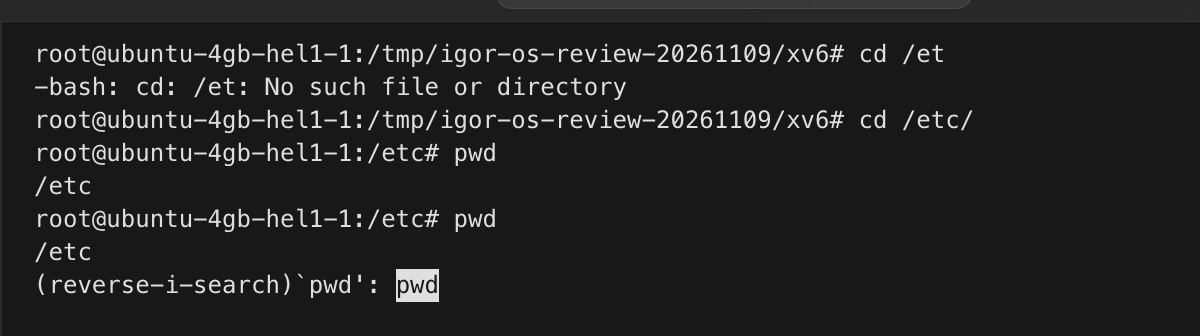
\includegraphics[width=\linewidth,height=0.67\textheight,keepaspectratio]{Lab3-4/evidence/screenshots/lab3-1.1.png}
\end{minipage}\par\medskip

\par\medskip\noindent\begin{minipage}{\linewidth}\setstretch{1.0}
\captionof*{figure}{Figura 1.2 – Type and which}
\centering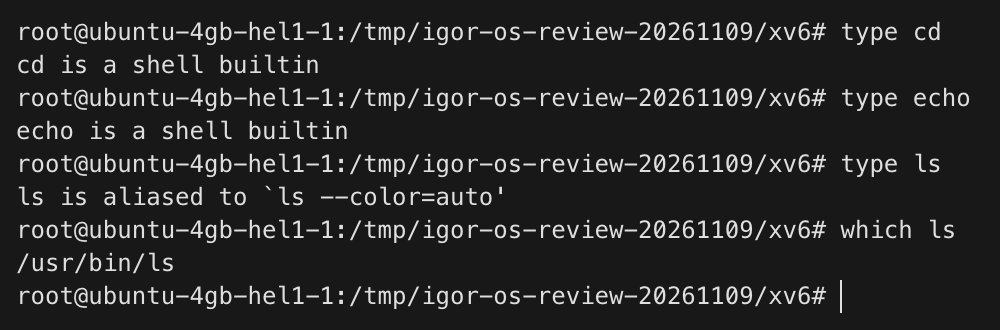
\includegraphics[width=\linewidth,height=0.67\textheight,keepaspectratio]{Lab3-4/evidence/screenshots/lab3-1.2.png}
\end{minipage}\par\medskip

\par\medskip\noindent\begin{minipage}{\linewidth}\setstretch{1.0}
\captionof*{figure}{Figura 1.3 – Directories in PATH}
\centering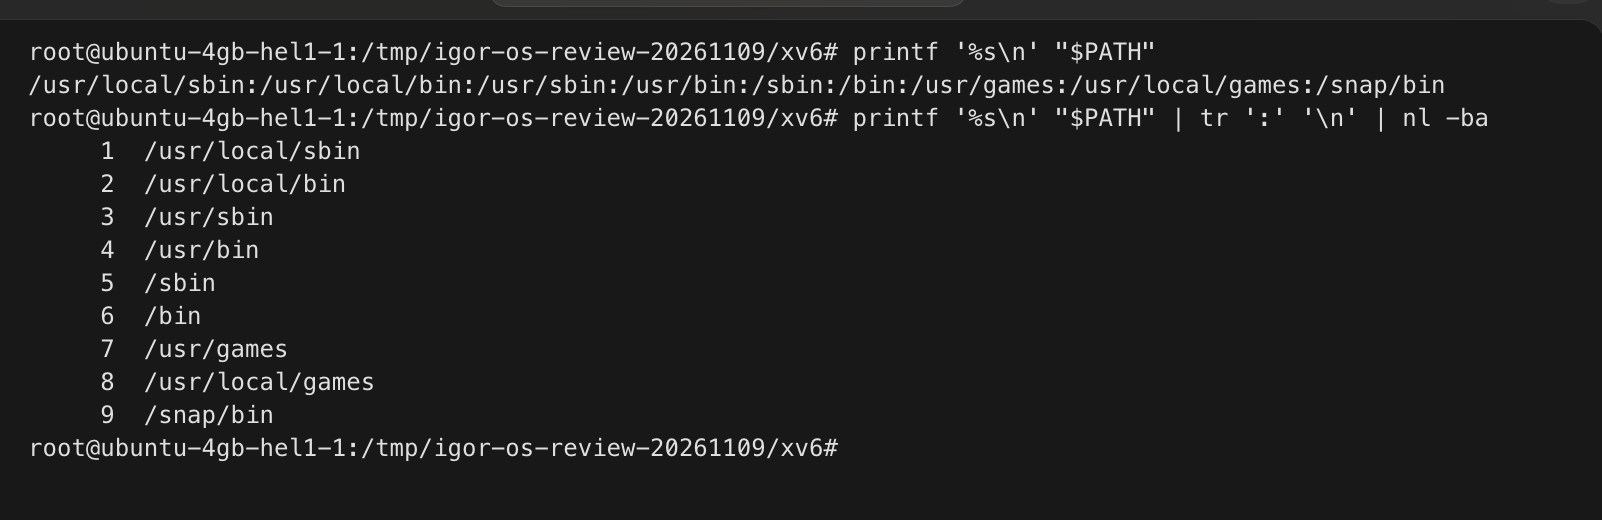
\includegraphics[width=\linewidth,height=0.67\textheight,keepaspectratio]{Lab3-4/evidence/screenshots/lab3-1.3.png}
\end{minipage}\par\medskip

\par\medskip\noindent\begin{minipage}{\linewidth}\setstretch{1.0}
\captionof*{figure}{Figura 1.4 – Exit status of a missing command}
\centering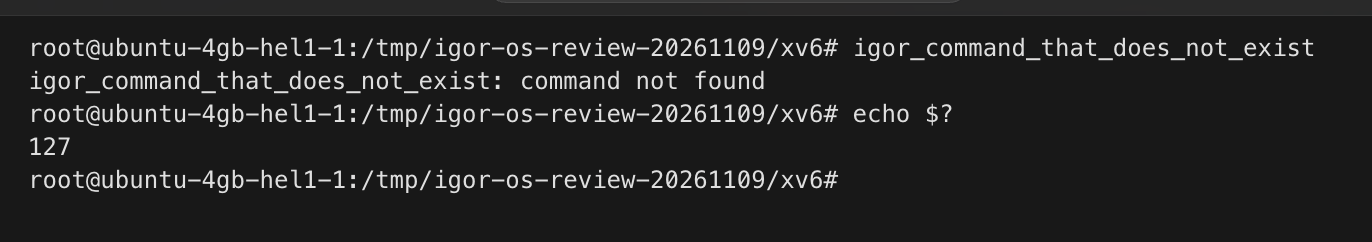
\includegraphics[width=\linewidth,height=0.67\textheight,keepaspectratio]{Lab3-4/evidence/screenshots/lab3-1.4.png}
\end{minipage}\par\medskip

\subsection{Part 2 Predictions and shell
expansion}\label{lab3-part-2-predictions-and-shell-expansion}

The required play directory contained a.c, b.c, file1.txt, file2.txt,
notes.txt and alfa beta.txt. Each prediction below was recorded before
execution; timestamps and complete stderr are retained in the JSON
evidence. Differences in line layout from ls are presentation
differences, not additional filenames.

{\def\LTcaptype{table} % do not increment counter
\begin{longtable}[]{@{}
  >{\raggedright\arraybackslash}p{(\linewidth - 6\tabcolsep) * \real{0.2500}}
  >{\raggedright\arraybackslash}p{(\linewidth - 6\tabcolsep) * \real{0.2500}}
  >{\raggedright\arraybackslash}p{(\linewidth - 6\tabcolsep) * \real{0.2500}}
  >{\raggedright\arraybackslash}p{(\linewidth - 6\tabcolsep) * \real{0.2500}}@{}}
\toprule\noalign{}
\begin{minipage}[b]{\linewidth}\raggedright
\textbf{Command}
\end{minipage} & \begin{minipage}[b]{\linewidth}\raggedright
\textbf{Prediction before run}
\end{minipage} & \begin{minipage}[b]{\linewidth}\raggedright
\textbf{Observed output and status}
\end{minipage} & \begin{minipage}[b]{\linewidth}\raggedright
\textbf{Explanation}
\end{minipage} \\
\midrule\noalign{}
\endhead
\bottomrule\noalign{}
\endlastfoot
echo *.c & a.c b.c & \begin{minipage}[t]{\linewidth}\raggedright
a.c b.c\\
status 0\strut
\end{minipage} & Bash expands the pattern before echo starts. \\
echo file?.txt & file1.txt file2.txt &
\begin{minipage}[t]{\linewidth}\raggedright
file1.txt file2.txt\\
status 0\strut
\end{minipage} & Question mark matches one character. \\
echo {[}a-b{]}* & a.c alfa beta.txt b.c &
\begin{minipage}[t]{\linewidth}\raggedright
a.c alfa beta.txt b.c\\
status 0\strut
\end{minipage} & The range matches names beginning with a or b. \\
echo *.xyz & literal *.xyz because no match exists &
\begin{minipage}[t]{\linewidth}\raggedright
*.xyz\\
status 0\strut
\end{minipage} & The unmatched pattern remains literal with the default
settings. \\
ls alfa beta.txt & two missing operands and a nonzero status &
\begin{minipage}[t]{\linewidth}\raggedright
ls: cannot access \textquotesingle alfa\textquotesingle: No such file or
directory\\
ls: cannot access \textquotesingle beta.txt\textquotesingle: No such
file or directory\\
status 2\strut
\end{minipage} & Unquoted whitespace creates two operands. \\
ls "alfa beta.txt" & one file named alfa beta.txt &
\begin{minipage}[t]{\linewidth}\raggedright
alfa beta.txt\\
status 0\strut
\end{minipage} & Quotes preserve one pathname containing a space. \\
echo \textquotesingle\$HOME\textquotesingle{} "\$HOME"
\textbackslash\$HOME & \$HOME /root \$HOME &
\begin{minipage}[t]{\linewidth}\raggedright
\$HOME /root \$HOME\\
status 0\strut
\end{minipage} & Single quotes and backslash protect the dollar sign;
double quotes permit expansion. \\
echo \{1..5\} ; echo \$((7 * 6)) & 1 2 3 4 5 then 42 &
\begin{minipage}[t]{\linewidth}\raggedright
1 2 3 4 5\\
42\\
status 0\strut
\end{minipage} & Brace expansion lists values; arithmetic expansion
computes 42. \\
echo "today is \$(date +\%A), I am \$(whoami)" & current weekday and
current login identity & \begin{minipage}[t]{\linewidth}\raggedright
today is Monday, I am root\\
status 0\strut
\end{minipage} & Command substitution supplies the current weekday and
identity. \\
touch log\{1..3\}.txt \&\& ls log* & log1.txt, log2.txt, log3.txt &
\begin{minipage}[t]{\linewidth}\raggedright
log1.txt\\
log2.txt\\
log3.txt\\
status 0\strut
\end{minipage} & Brace expansion creates three filenames. \\
\end{longtable}
}

Echo does not discover files; Bash supplies the expanded arguments. The
unquoted space in ls alfa beta.txt produces two failed lookups. Both ls
"alfa beta.txt" and ls alfa\textbackslash{} beta.txt address the single
file correctly. Single quotes retain literal text; double quotes still
allow parameter and command substitution. GNU ls may display quotes for
a space-containing filename when its output is a terminal, but those
display quotes are not stored in the name.

\par\medskip\noindent\begin{minipage}{\linewidth}\setstretch{1.0}
\captionof*{figure}{Figura 2.1 – Files in the required play directory}
\centering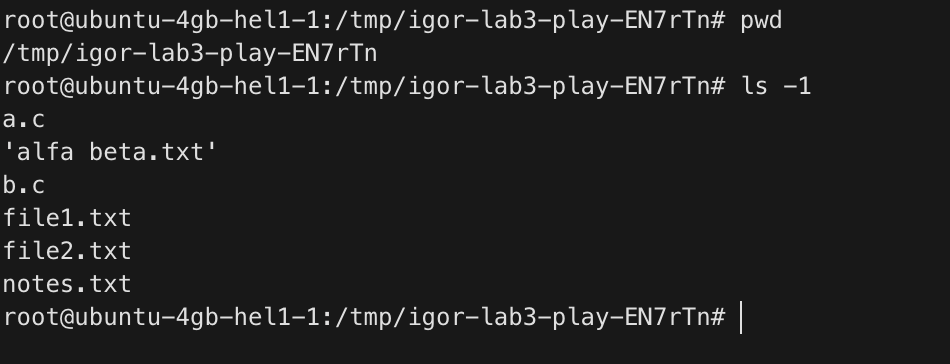
\includegraphics[width=\linewidth,height=0.67\textheight,keepaspectratio]{Lab3-4/evidence/screenshots/lab3-2.1.png}
\end{minipage}\par\medskip

\par\medskip\noindent\begin{minipage}{\linewidth}\setstretch{1.0}
\captionof*{figure}{Figura 2.2 – Globbing results}
\centering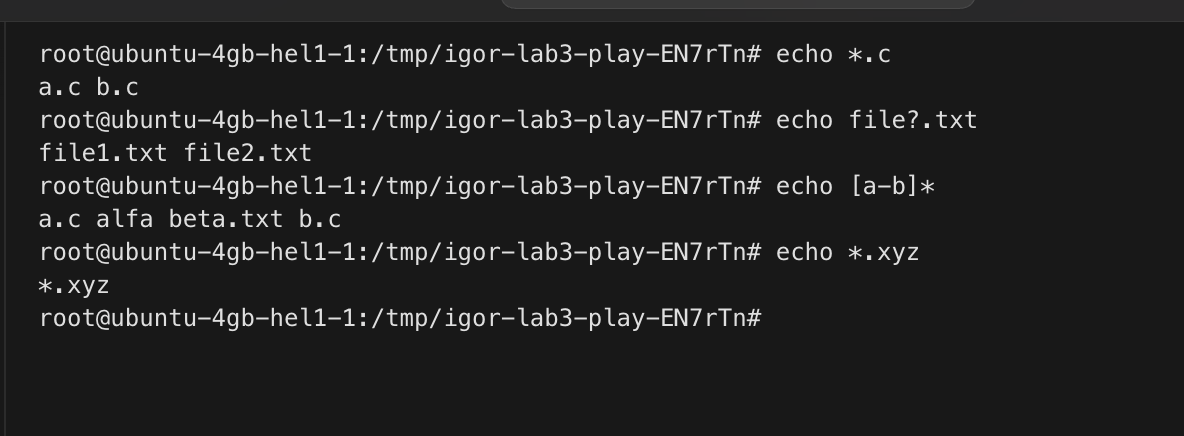
\includegraphics[width=\linewidth,height=0.67\textheight,keepaspectratio]{Lab3-4/evidence/screenshots/lab3-2.2.png}
\end{minipage}\par\medskip

\par\medskip\noindent\begin{minipage}{\linewidth}\setstretch{1.0}
\captionof*{figure}{Figura 2.3 – A space containing name and the quoted fix}
\centering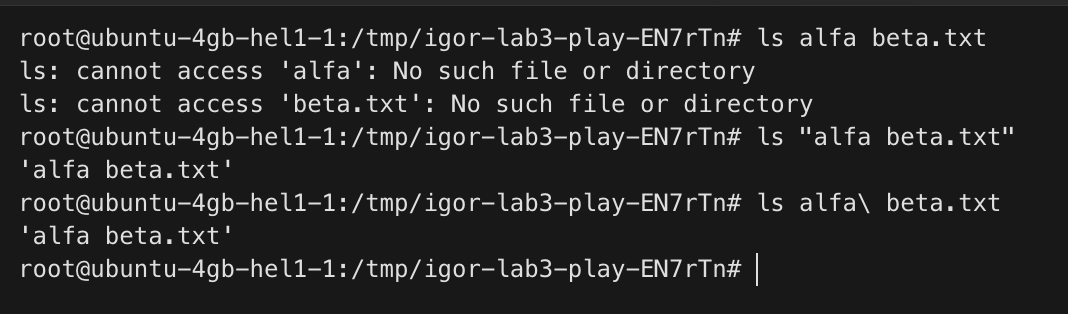
\includegraphics[width=\linewidth,height=0.67\textheight,keepaspectratio]{Lab3-4/evidence/screenshots/lab3-2.3.png}
\end{minipage}\par\medskip

\par\medskip\noindent\begin{minipage}{\linewidth}\setstretch{1.0}
\captionof*{figure}{Figura 2.4 – Single double and escaped dollar quoting}
\centering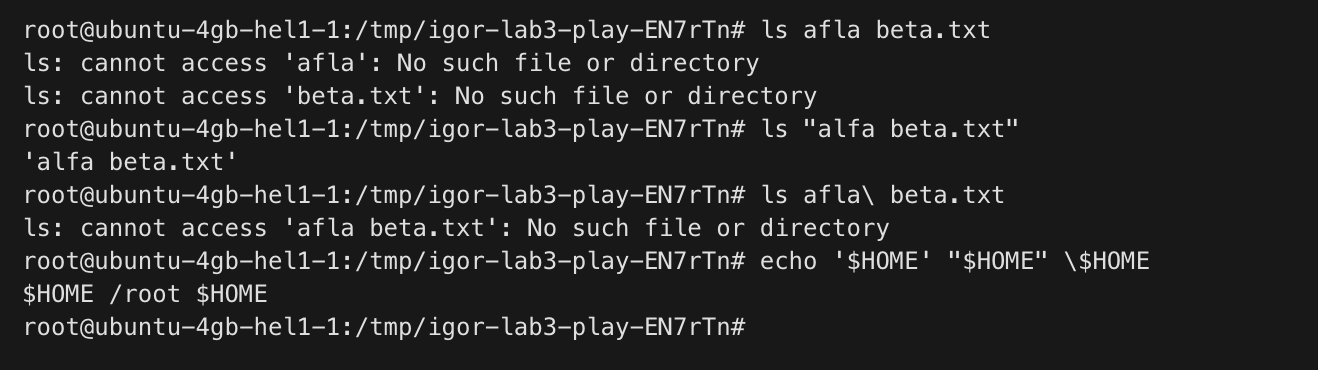
\includegraphics[width=\linewidth,height=0.67\textheight,keepaspectratio]{Lab3-4/evidence/screenshots/lab3-2.4.png}
\end{minipage}\par\medskip

\subsection{Part 3 Redirection chaining and
jobs}\label{lab3-part-3-redirection-chaining-and-jobs}

Out.txt received stdout, while err.txt received the diagnostic for
/nope. In \textgreater{} all.txt 2\textgreater\&1, descriptor 1 is
changed first and descriptor 2 duplicates that new target. In
2\textgreater\&1 \textgreater{} all.txt, stderr keeps the original
stdout target while only stdout moves to the file. Wc -l \textless{}
access.log receives stdin and therefore prints a count only; with
access.log as an operand it also knows and prints the filename. A
semicolon sequences regardless of the previous status; AND runs the next
command only after success; OR runs it only after failure. The
background sleep was listed, terminated and reaped with status 143.

\par\medskip\noindent\begin{minipage}{\linewidth}\setstretch{1.0}
\captionof*{figure}{Figura 3.1 – Stdout and stderr in separate files}
\centering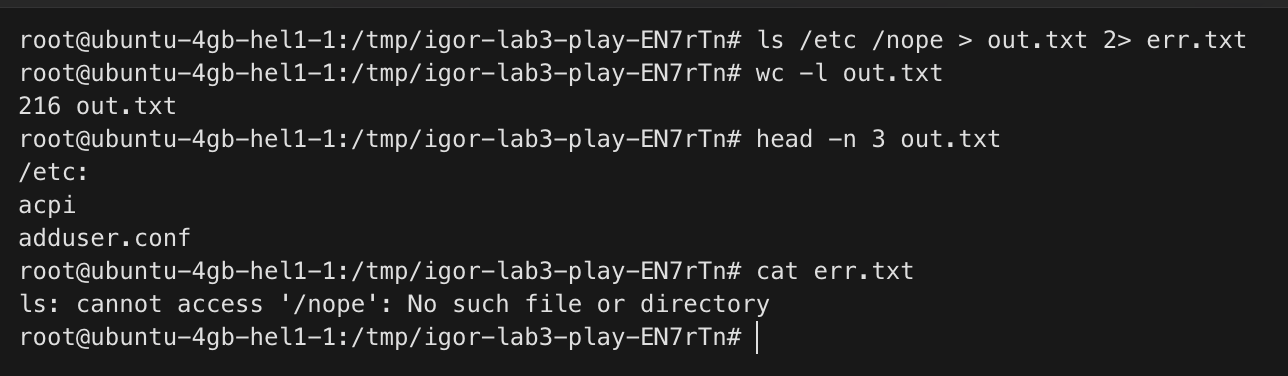
\includegraphics[width=\linewidth,height=0.67\textheight,keepaspectratio]{Lab3-4/evidence/screenshots/lab3-3.1.png}
\end{minipage}\par\medskip

\par\medskip\noindent\begin{minipage}{\linewidth}\setstretch{1.0}
\captionof*{figure}{Figura 3.2 – Order of descriptor redirections}
\centering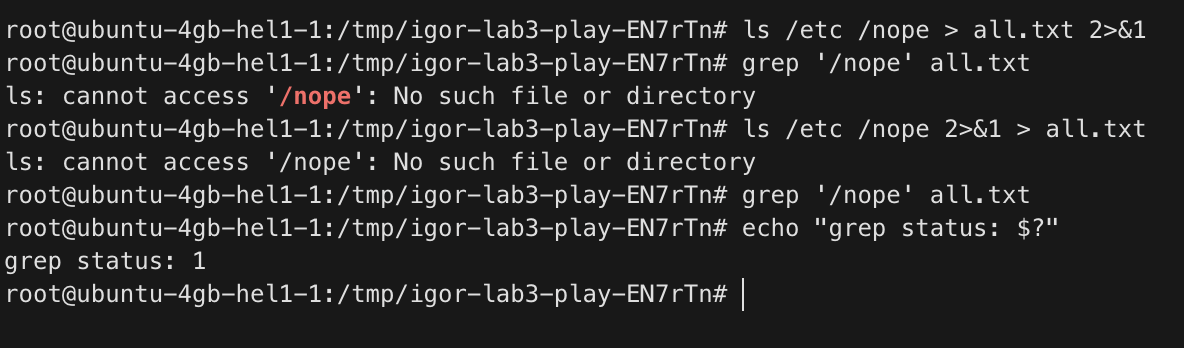
\includegraphics[width=\linewidth,height=0.67\textheight,keepaspectratio]{Lab3-4/evidence/screenshots/lab3-3.2.png}
\end{minipage}\par\medskip

\par\medskip\noindent\begin{minipage}{\linewidth}\setstretch{1.0}
\captionof*{figure}{Figura 3.3 – Semicolon AND and OR}
\centering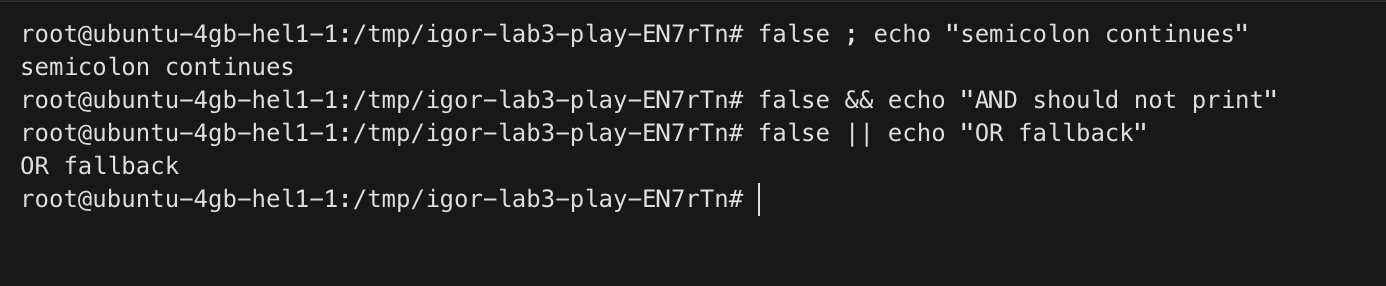
\includegraphics[width=\linewidth,height=0.67\textheight,keepaspectratio]{Lab3-4/evidence/screenshots/lab3-3.3.png}
\end{minipage}\par\medskip

\par\medskip\noindent\begin{minipage}{\linewidth}\setstretch{1.0}
\captionof*{figure}{Figura 3.4 – Background job and termination}
\centering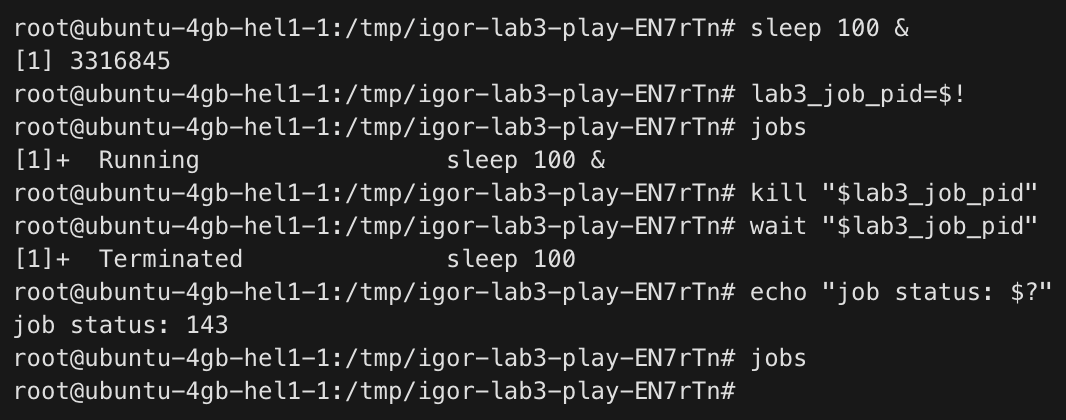
\includegraphics[width=\linewidth,height=0.67\textheight,keepaspectratio]{Lab3-4/evidence/screenshots/lab3-3.4.png}
\end{minipage}\par\medskip

\subsection{Part 4 Answers to the eight log
questions}\label{lab3-part-4-answers-to-the-eight-log-questions}

The artificial dataset uses the exact 2026-10-05 generator supplied in
the handout. It is shared assignment input rather than real web traffic.
All 500 lines were regenerated. The pipelines compare the result field,
preserve tied maxima and sort their output. The four page counts sum to
500 and the seven user failure counts sum to 100. In Q8 the long listing
has one extra total header line; the entries are otherwise the same.

\par\medskip\noindent\begin{minipage}{\linewidth}\setstretch{1.0}
\captionof*{figure}{Figura 4.1–4.2 – Questions 1 and 2 results}
\centering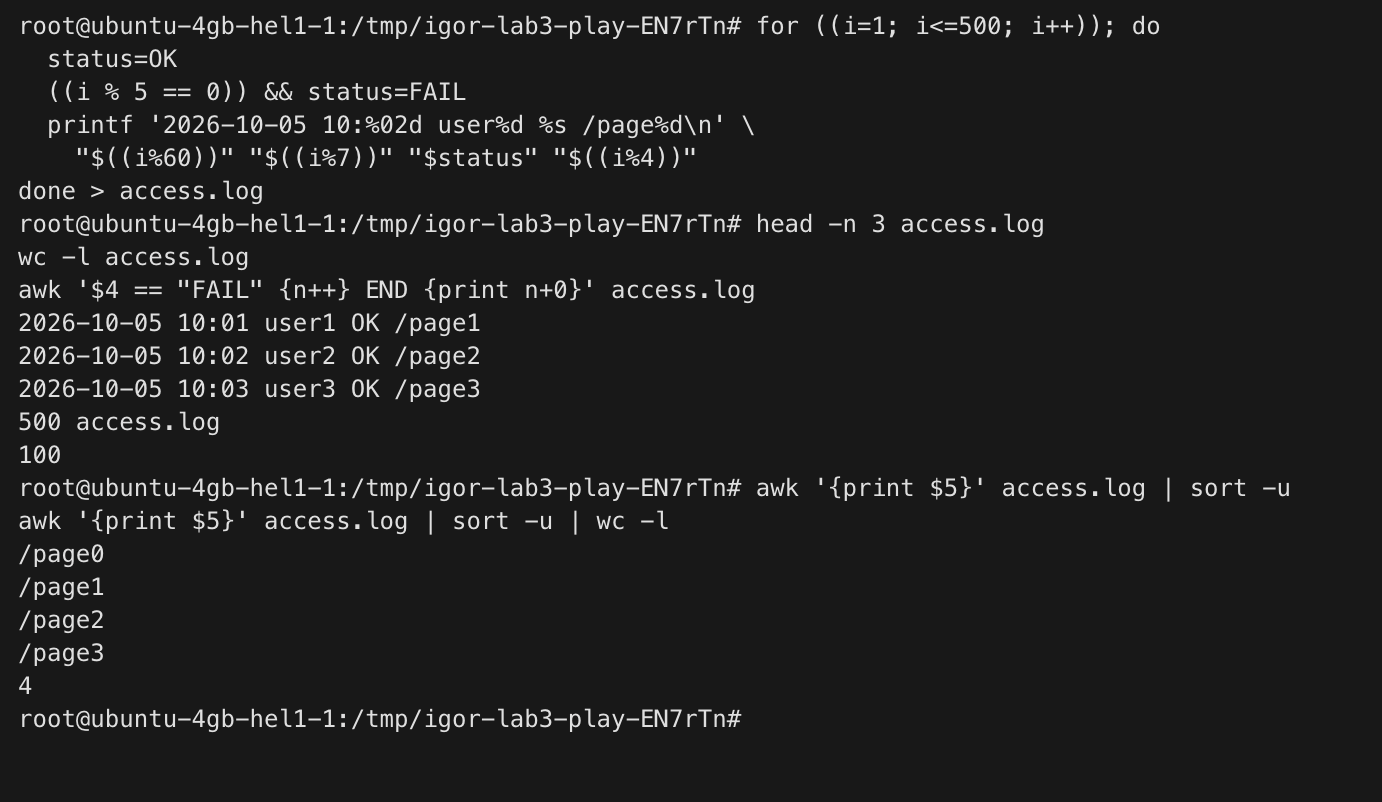
\includegraphics[width=\linewidth,height=0.67\textheight,keepaspectratio]{Lab3-4/evidence/screenshots/lab3-4.1-4.2.png}
\end{minipage}\par\medskip

\par\medskip\noindent\begin{minipage}{\linewidth}\setstretch{1.0}
\captionof*{figure}{Figura 4.3–4.4 – Questions 3 and 4 results}
\centering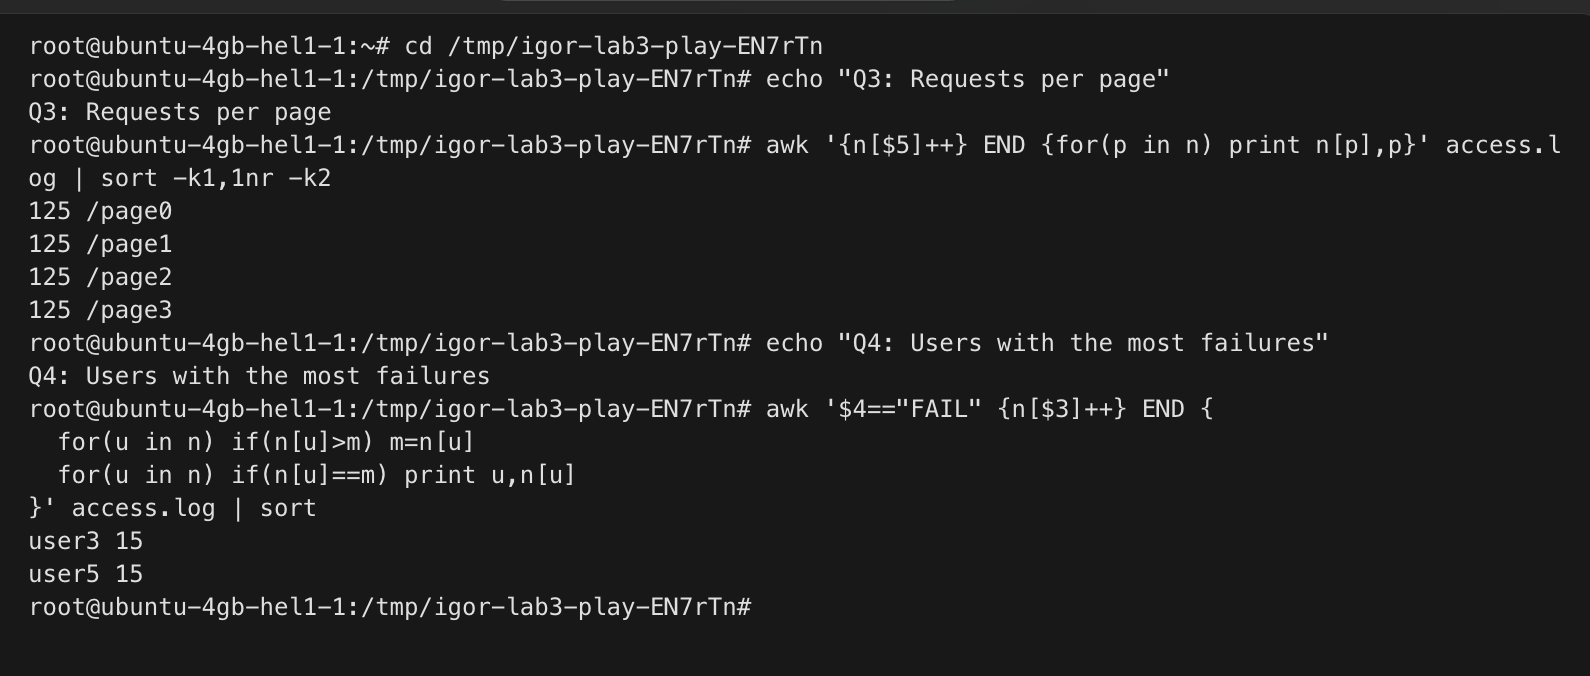
\includegraphics[width=\linewidth,height=0.67\textheight,keepaspectratio]{Lab3-4/evidence/screenshots/lab3-4.3-4.4.png}
\end{minipage}\par\medskip

\par\medskip\noindent\begin{minipage}{\linewidth}\setstretch{1.0}
\captionof*{figure}{Figura 4.5–4.6 – Questions 5 and 6 results}
\centering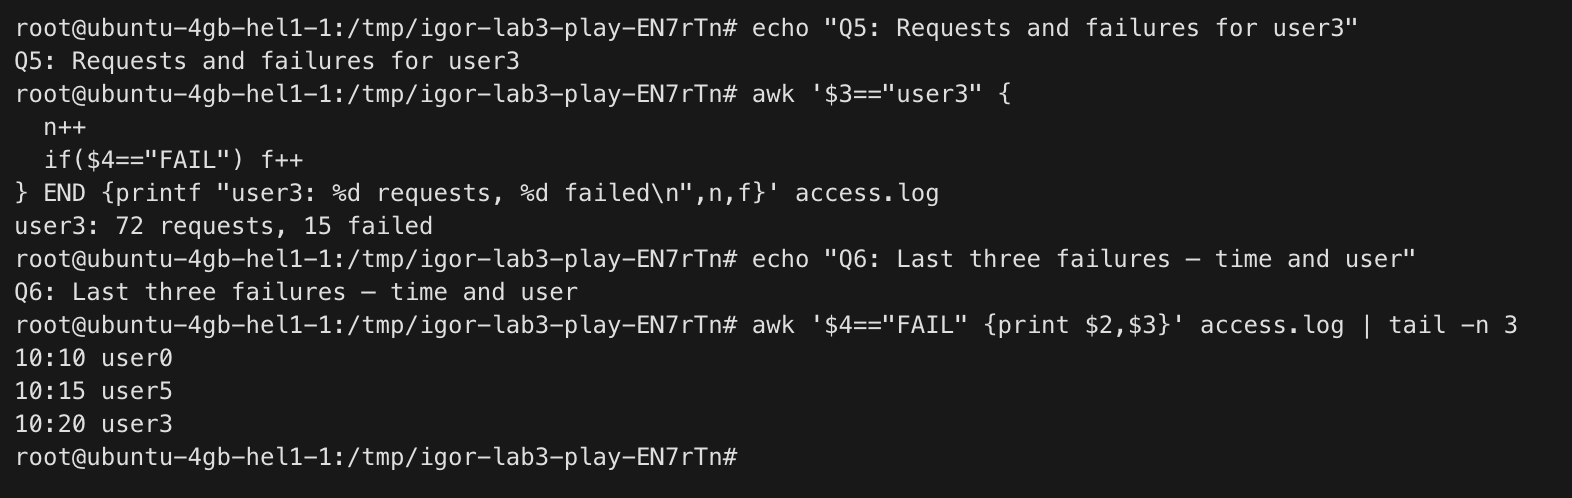
\includegraphics[width=\linewidth,height=0.67\textheight,keepaspectratio]{Lab3-4/evidence/screenshots/lab3-4.5-4.6.png}
\end{minipage}\par\medskip

\par\medskip\noindent\begin{minipage}{\linewidth}\setstretch{1.0}
\captionof*{figure}{Figura 4.7–4.8 – Questions 7 and 8 results}
\centering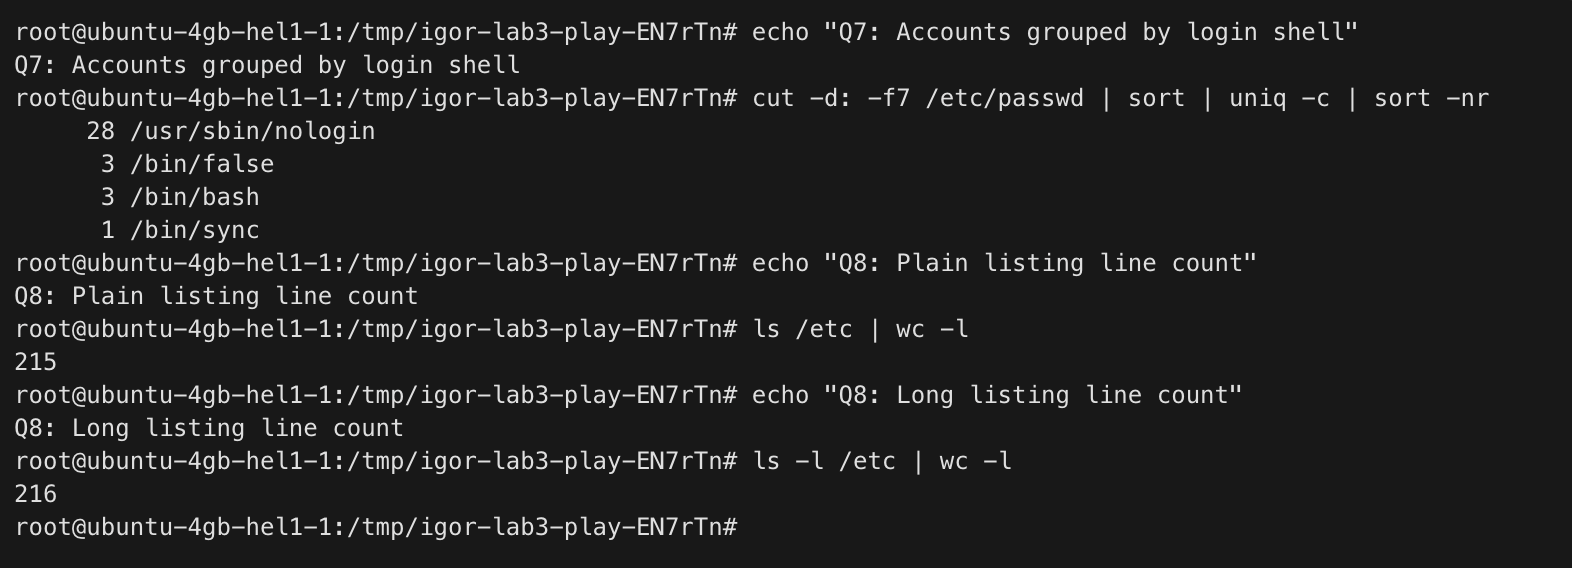
\includegraphics[width=\linewidth,height=0.67\textheight,keepaspectratio]{Lab3-4/evidence/screenshots/lab3-4.7-4.8.png}
\end{minipage}\par\medskip

\par\medskip\noindent\begin{minipage}{\linewidth}\setstretch{1.0}
\captionof*{figure}{Figura 4.9 – Full run of oneliners.sh}
\centering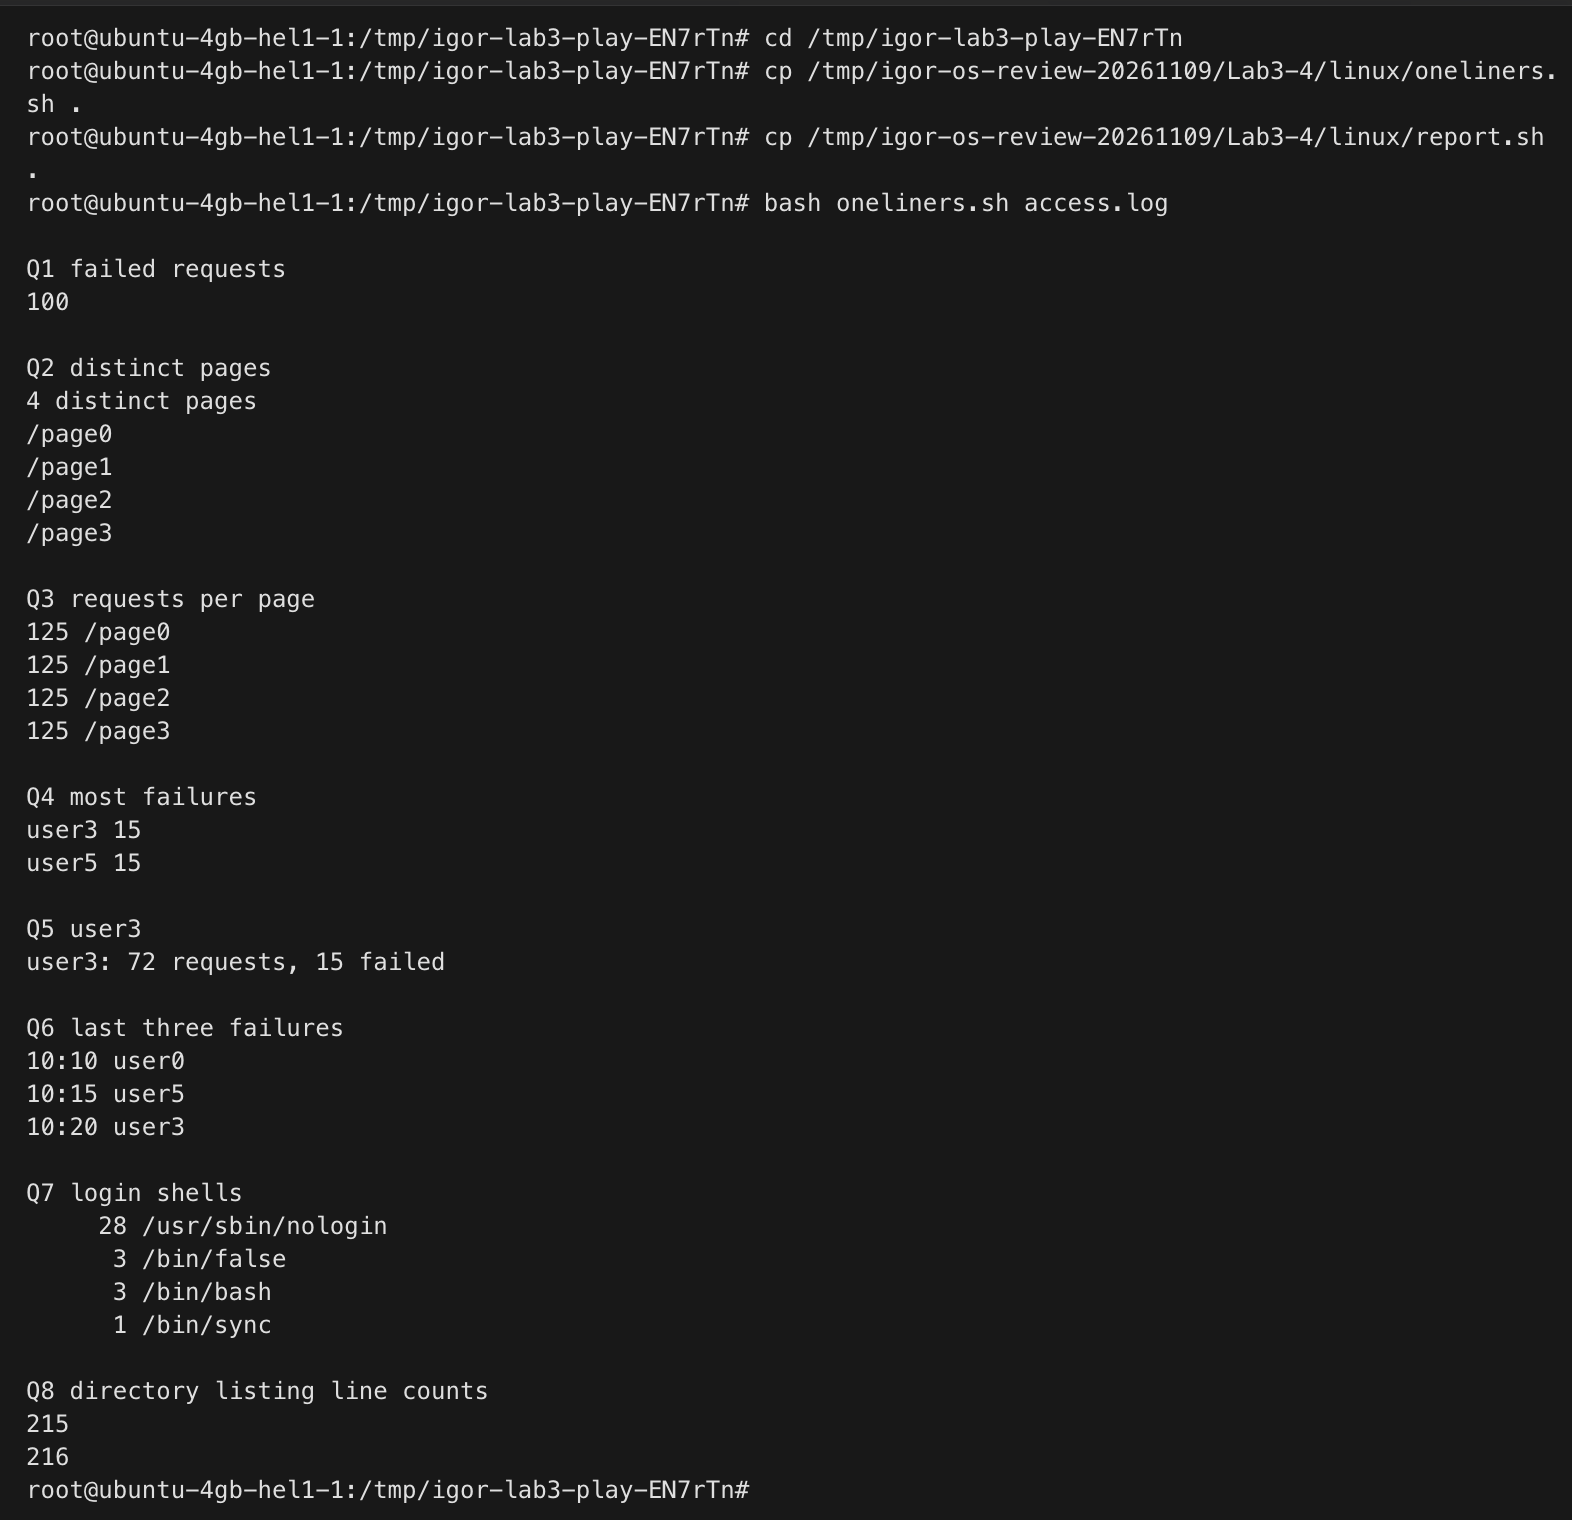
\includegraphics[width=\linewidth,height=0.67\textheight,keepaspectratio]{Lab3-4/evidence/screenshots/lab3-4.9.png}
\end{minipage}\par\medskip

\subsection{Part 5 The report script and its error
path}\label{lab3-part-5-the-report-script-and-its-error-path}

The shebang \#!/bin/bash selects Bash when the executable script is
launched directly. Before chmod +x, ./report.sh returned permission
denied and status 126. The prefix ./ supplies a pathname because the
current directory is not searched through PATH here. The error is
written to descriptor 2 so stdout remains usable for normal results;
exit 1 lets a caller detect failure. The script prints every user from
user0 to user6, including zero counts, using its aggregation loop.
Optional cron and bonus tasks are not claimed.

\par\medskip\noindent\begin{minipage}{\linewidth}\setstretch{1.0}
\captionof*{figure}{Figura 5.1 – Source of report.sh}
\centering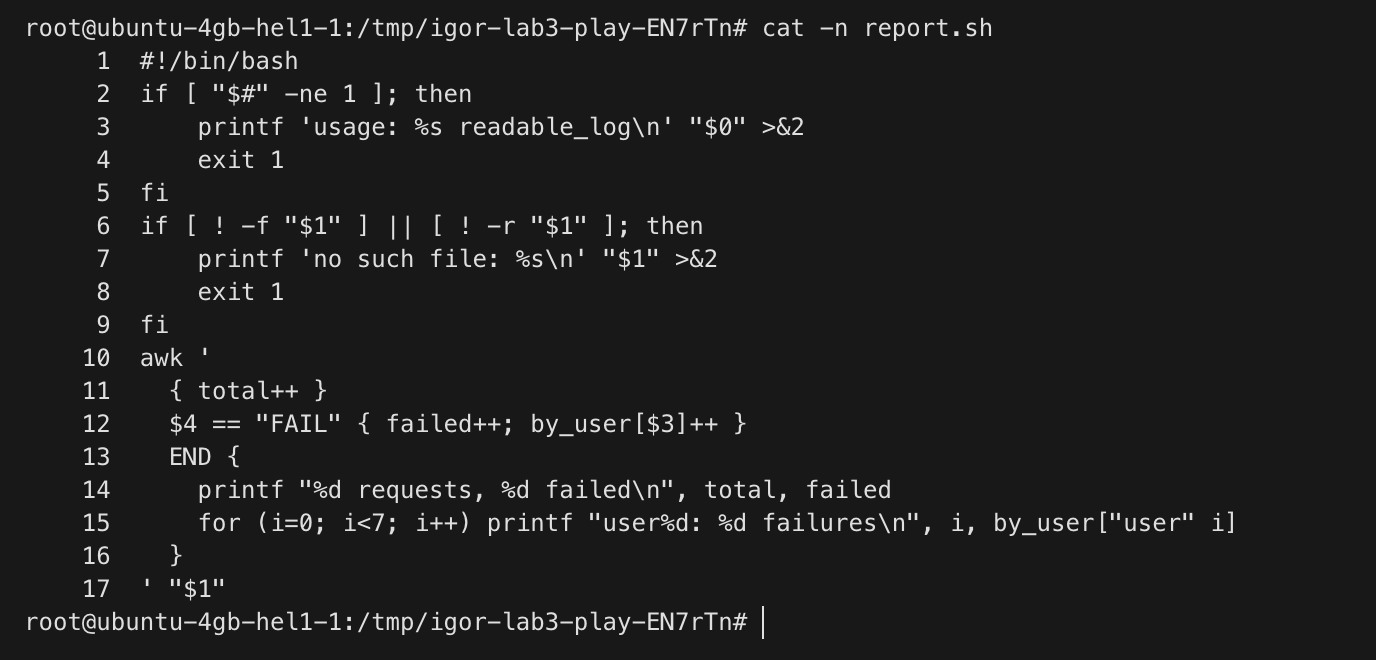
\includegraphics[width=\linewidth,height=0.67\textheight,keepaspectratio]{Lab3-4/evidence/screenshots/lab3-5.1.png}
\end{minipage}\par\medskip

\par\medskip\noindent\begin{minipage}{\linewidth}\setstretch{1.0}
\captionof*{figure}{Figura 5.2 – Successful report and execute permission check}
\centering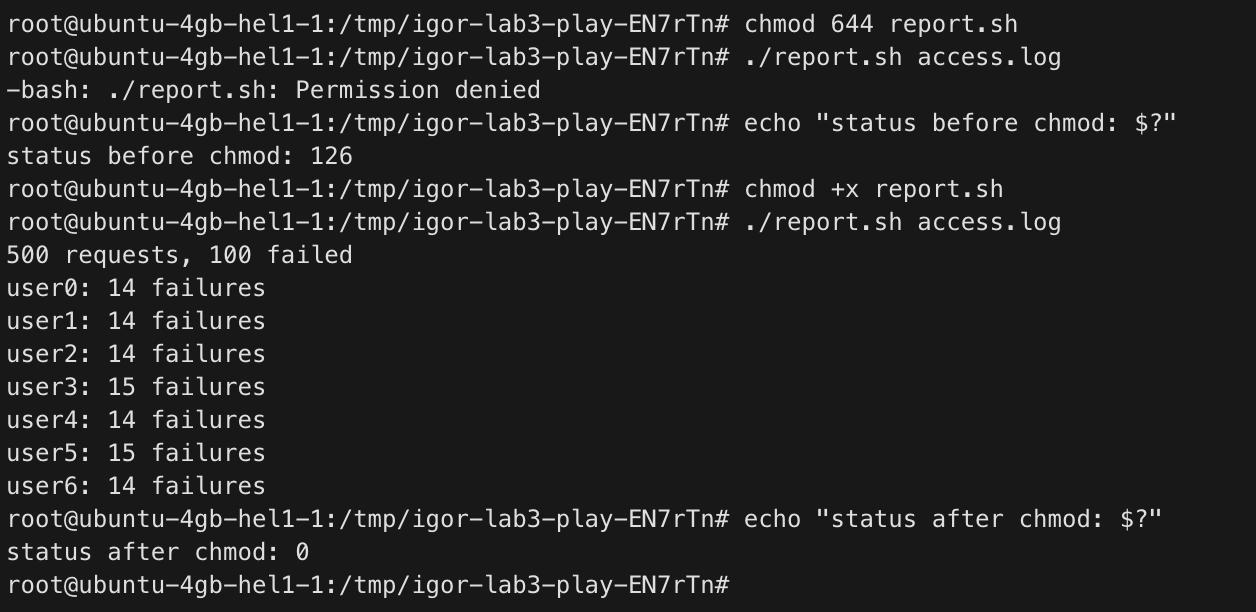
\includegraphics[width=\linewidth,height=0.67\textheight,keepaspectratio]{Lab3-4/evidence/screenshots/lab3-5.2.png}
\end{minipage}\par\medskip

\par\medskip\noindent\begin{minipage}{\linewidth}\setstretch{1.0}
\captionof*{figure}{Figura 5.3 – Missing file diagnostic and status}
\centering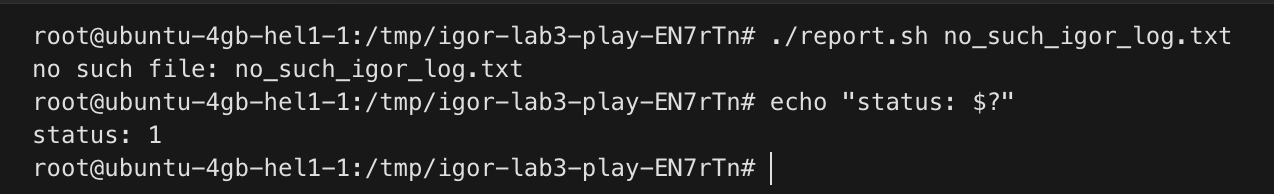
\includegraphics[width=\linewidth,height=0.67\textheight,keepaspectratio]{Lab3-4/evidence/screenshots/lab3-5.3.png}
\end{minipage}\par\medskip

\subsection{Concluziile laboratorului 3}\label{lab3-concluzie}

Argument expansion belongs to Bash before program execution. Descriptor
duplication explains the order-sensitive redirection result, while
status-dependent operators make failure handling explicit. The
one-liners were verified against fixed input totals and the reusable
script was tested on success and missing input. Source files,
predictions and raw recordings accompany this report.

\subsection{Laboratorul 4}\label{laboratorul-4}

\subsection{Purpose and execution
record}\label{lab4-purpose-and-execution-record}

All twelve figures are native Terminal screenshots supplied by the
author from direct command execution and source inspection on the Ubuntu
server on 9 November 2026. The xv6 tests use an isolated source copy and
its generated test disk. The directory d already existed during the
directory-handling capture; grep READ limits the displayed listing. Bash
comparisons use separate temporary directories. Source files and earlier
full execution transcripts accompany the screenshots. The submission was
prepared with coding assistance; MIT xv6 is identified as upstream in
the source provenance file.

\subsection{Part 1 Sleep and the current
interface}\label{lab4-part-1-sleep-and-the-current-interface}

The header declares pause rather than sleep. The submitted utility calls
pause with validated decimal ticks; sleep 20 returns normally, missing
input produces usage, and negative input produces a diagnostic. The
Makefile contains the \_sleep entry. Forked processes inherit the binary
and descriptor context, while pause is the kernel operation that
performs the delay.

\par\medskip\noindent\begin{minipage}{\linewidth}\setstretch{1.0}
\captionof*{figure}{Figura 1.1 – The pause declaration}
\centering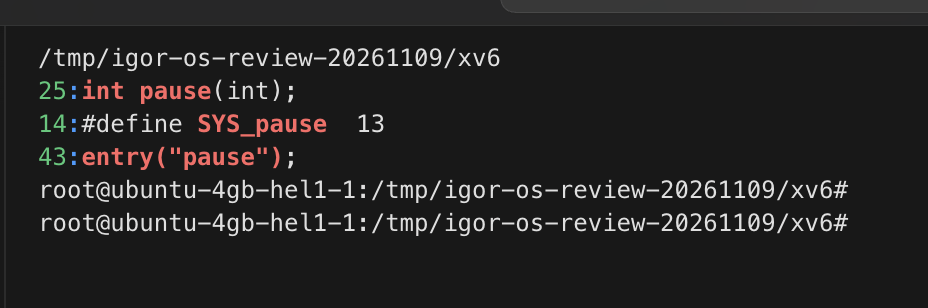
\includegraphics[width=\linewidth,height=0.67\textheight,keepaspectratio]{Lab3-4/evidence/screenshots/lab4-1.1.png}
\end{minipage}\par\medskip

\par\medskip\noindent\begin{minipage}{\linewidth}\setstretch{1.0}
\captionof*{figure}{Figura 1.2 – Sleep source and registration}
\centering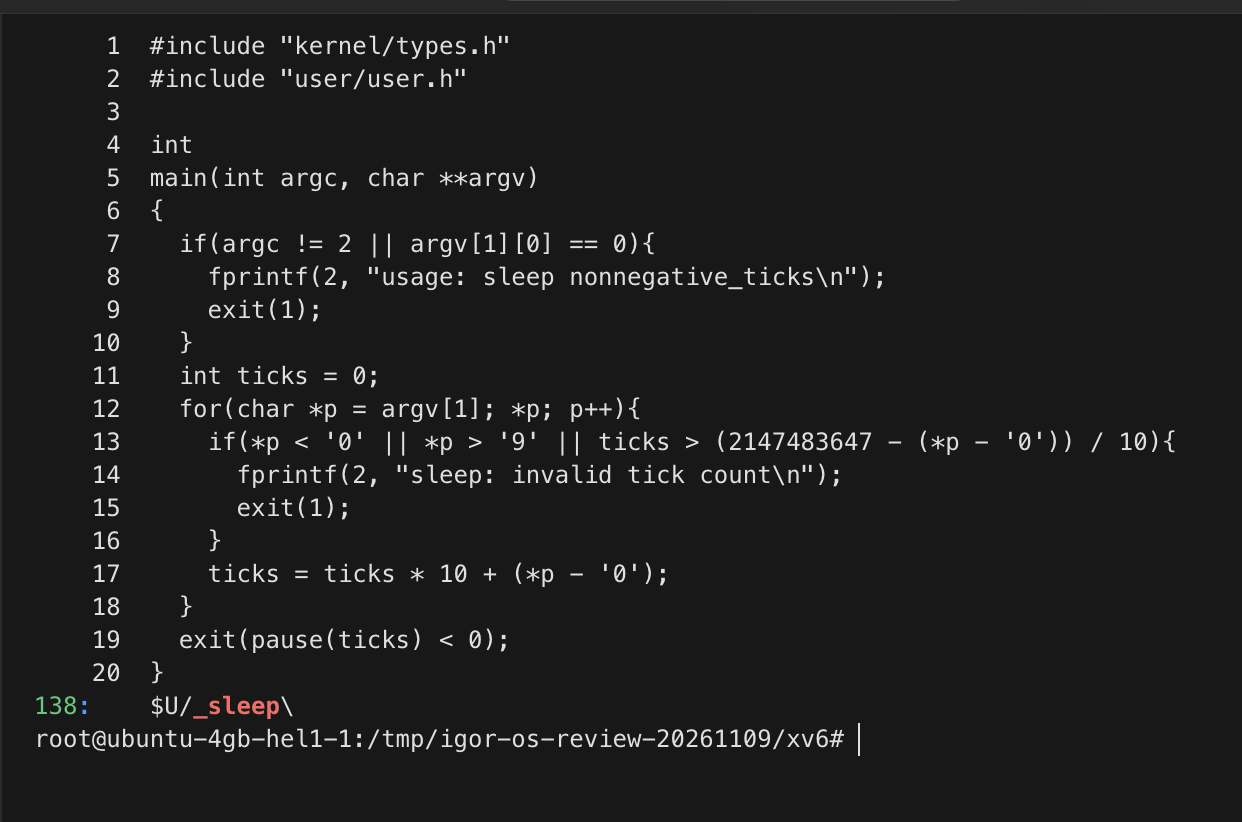
\includegraphics[width=\linewidth,height=0.67\textheight,keepaspectratio]{Lab3-4/evidence/screenshots/lab4-1.2.png}
\end{minipage}\par\medskip

\par\medskip\noindent\begin{minipage}{\linewidth}\setstretch{1.0}
\captionof*{figure}{Figura 1.3 – Sleep with valid and invalid arguments}
\centering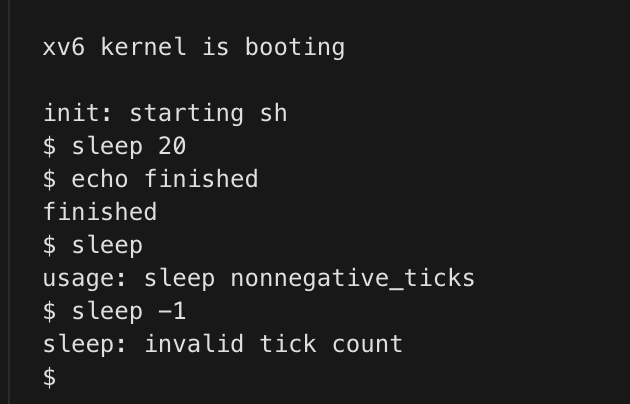
\includegraphics[width=\linewidth,height=0.67\textheight,keepaspectratio]{Lab3-4/evidence/screenshots/lab4-1.3.png}
\end{minipage}\par\medskip

\subsection{Part 2 Comparing every command in the two
shells}\label{lab4-part-2-comparing-every-command-in-the-two-shells}

The Bash test starts in a fresh directory containing README. Both shells
provide execution, descriptor redirection, pipelines, command lists,
grouping and background commands. Bash additionally expands wildcards
and variables, removes syntactic quotes, and offers readline history and
completion. The table records the actual small-shell behavior rather
than assuming it implements Bash syntax.

{\def\LTcaptype{table} % do not increment counter
\begin{longtable}[]{@{}
  >{\raggedright\arraybackslash}p{(\linewidth - 6\tabcolsep) * \real{0.2500}}
  >{\raggedright\arraybackslash}p{(\linewidth - 6\tabcolsep) * \real{0.2500}}
  >{\raggedright\arraybackslash}p{(\linewidth - 6\tabcolsep) * \real{0.2500}}
  >{\raggedright\arraybackslash}p{(\linewidth - 6\tabcolsep) * \real{0.2500}}@{}}
\toprule\noalign{}
\begin{minipage}[b]{\linewidth}\raggedright
\textbf{Command}
\end{minipage} & \begin{minipage}[b]{\linewidth}\raggedright
\textbf{Bash}
\end{minipage} & \begin{minipage}[b]{\linewidth}\raggedright
\textbf{xv6}
\end{minipage} & \begin{minipage}[b]{\linewidth}\raggedright
\textbf{Reason}
\end{minipage} \\
\midrule\noalign{}
\endhead
\bottomrule\noalign{}
\endlastfoot
echo hello \textgreater{} f ; cat \textless{} f & hello & hello &
descriptor redirection \\
ls \textbar{} grep READ & README & README line & pipe \\
(echo a; echo b) \textbar{} wc & 2 lines 2 words 4 bytes & 2 2 4 & group
and list \\
echo one ; echo two & one then two & one then two & sequence \\
echo bg \& & bg and prompt & bg and prompt & background \\
ls * & expands existing names & cannot open * & Bash pathname
expansion \\
echo \$HOME & /root & \$HOME & Bash variable expansion \\
echo "a b" & a b & "a b" & Bash quote removal \\
mkdir d ; cd d ; ls .. & lists parent after changing directory & exec cd
failed; lists from original directory & xv6 handles cd only as a whole
input line \\
Up Tab Ctrl+R & history and completion & not implemented as Bash
readline features & source and PTY inspection \\
\end{longtable}
}

There is an important distinction in the last directory case. A cd
embedded in a semicolon list is passed through the xv6 execution parser
and fails as an external command. Issuing cd d as its own input line
does change the parent shell. From there a bare ls fails because xv6 has
no PATH search, while /ls .. succeeds. For interactive work, history and
completion are valuable additions. Basic quote handling would be a
localized tokenizer improvement; full pathname expansion would also
require directory traversal.

\par\medskip\noindent\begin{minipage}{\linewidth}\setstretch{1.0}
\captionof*{figure}{Figura 2.1 – The original comparison commands in Bash}
\centering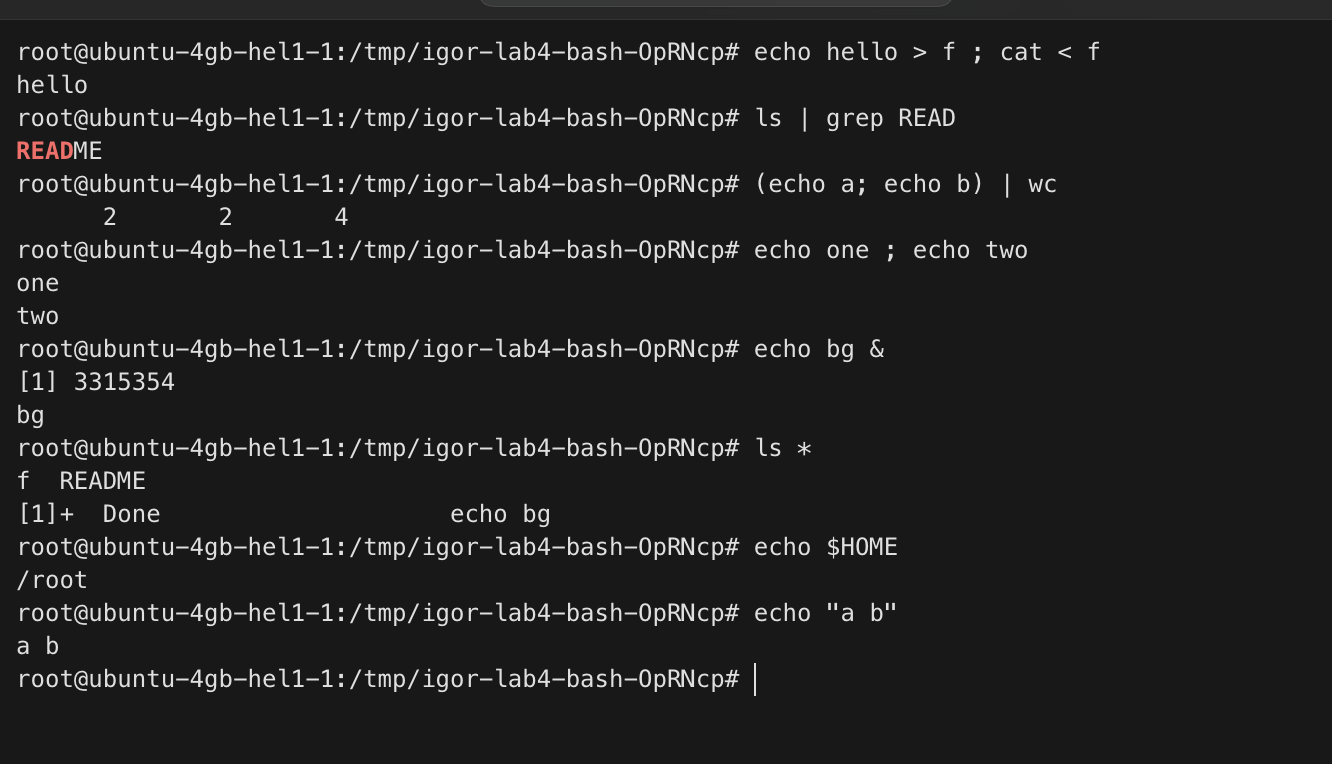
\includegraphics[width=\linewidth,height=0.67\textheight,keepaspectratio]{Lab3-4/evidence/screenshots/lab4-2.1.png}
\end{minipage}\par\medskip

\par\medskip\noindent\begin{minipage}{\linewidth}\setstretch{1.0}
\captionof*{figure}{Figura 2.2 – The same comparison commands in xv6}
\centering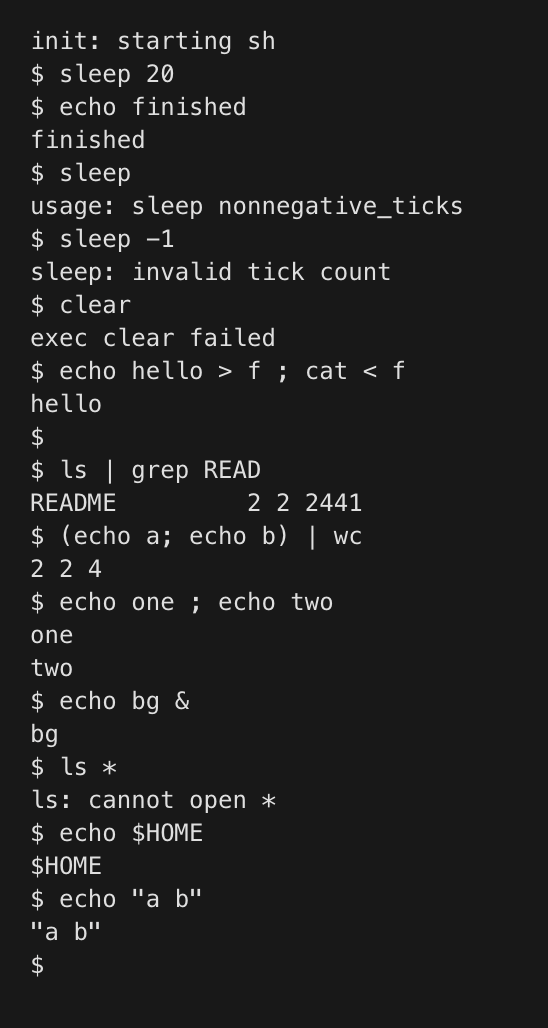
\includegraphics[width=\linewidth,height=0.67\textheight,keepaspectratio]{Lab3-4/evidence/screenshots/lab4-2.2.png}
\end{minipage}\par\medskip

\par\medskip\noindent\begin{minipage}{\linewidth}\setstretch{1.0}
\captionof*{figure}{Figura 2.3 – Directory handling and absolute ls (README-filtered listing)}
\centering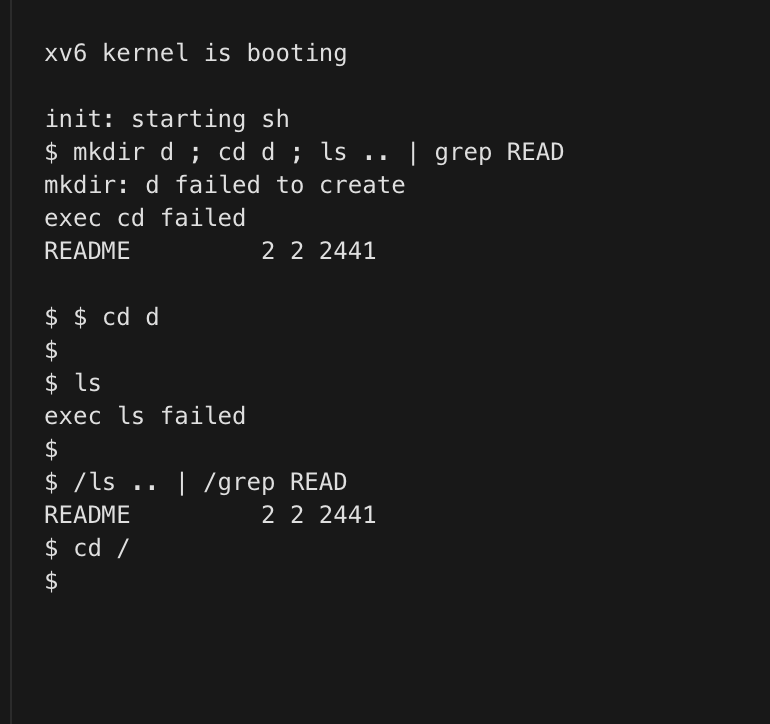
\includegraphics[width=\linewidth,height=0.67\textheight,keepaspectratio]{Lab3-4/evidence/screenshots/lab4-2.3.png}
\end{minipage}\par\medskip

\subsection{Part 3 Who expands the argument
vector}\label{lab4-part-3-who-expands-the-argument-vector}

Both inspectors print only argc and argv. The Linux wildcard experiment
in this additional test directory had four C files and one quoted x y
operand, giving argc 6 including argv zero. Xv6 passed four arguments:
args, the literal *.c, and two values containing the double quote marks.
The shell, not the inspector or kernel, is responsible for expansion and
syntactic quote removal. Repeated unquoted spaces delimit arguments in
both shells; they do not become empty arguments.

\par\medskip\noindent\begin{minipage}{\linewidth}\setstretch{1.0}
\captionof*{figure}{Figura 3.1 – Args source and UPROGS entry}
\centering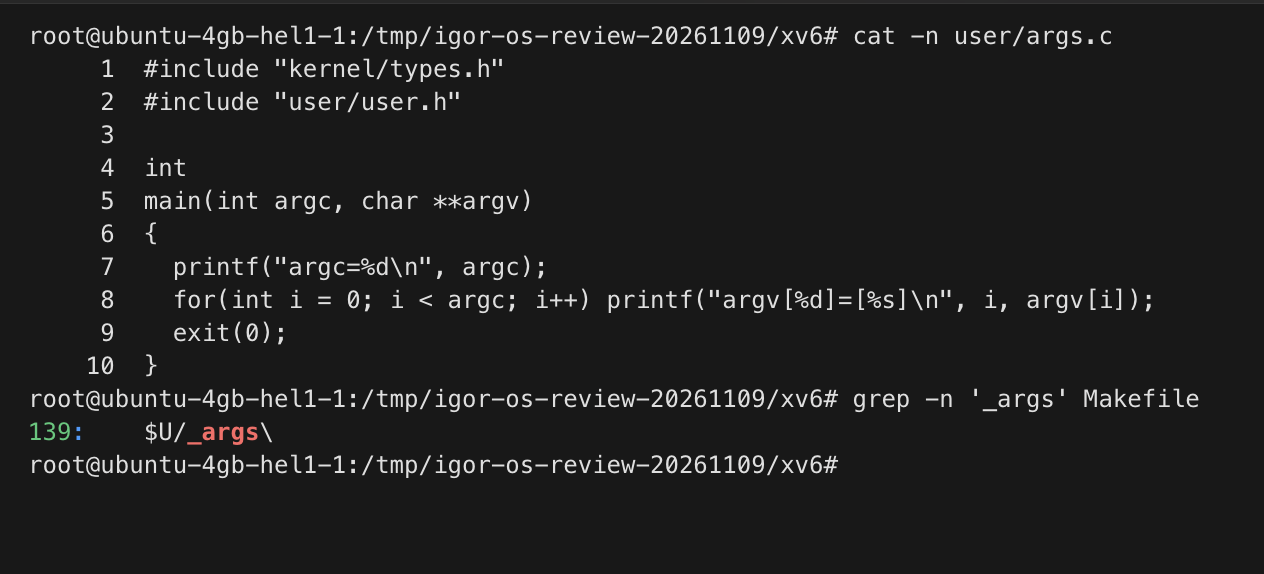
\includegraphics[width=\linewidth,height=0.67\textheight,keepaspectratio]{Lab3-4/evidence/screenshots/lab4-3.1.png}
\end{minipage}\par\medskip

\par\medskip\noindent\begin{minipage}{\linewidth}\setstretch{1.0}
\captionof*{figure}{Figura 3.2 – Argument arrays from xv6}
\centering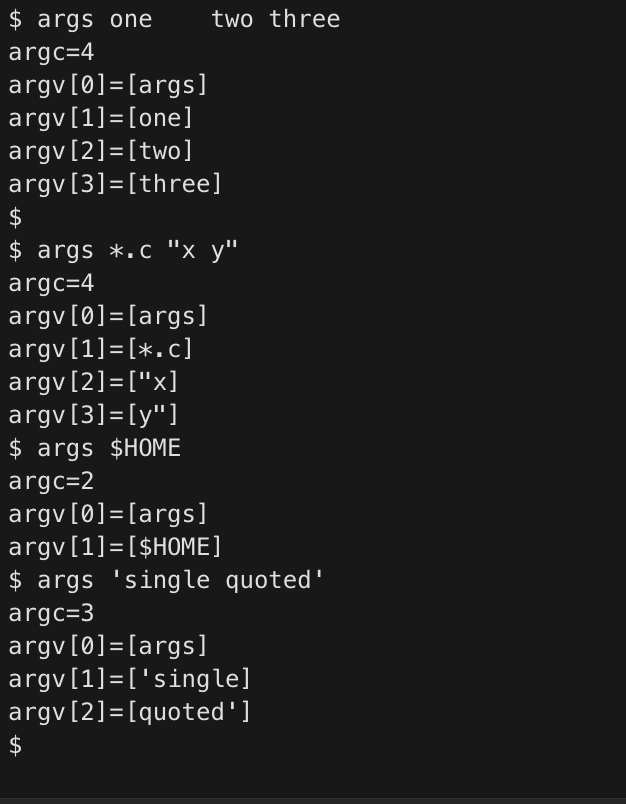
\includegraphics[width=\linewidth,height=0.67\textheight,keepaspectratio]{Lab3-4/evidence/screenshots/lab4-3.2.png}
\end{minipage}\par\medskip

\par\medskip\noindent\begin{minipage}{\linewidth}\setstretch{1.0}
\captionof*{figure}{Figura 3.3 – Argument arrays from Linux}
\centering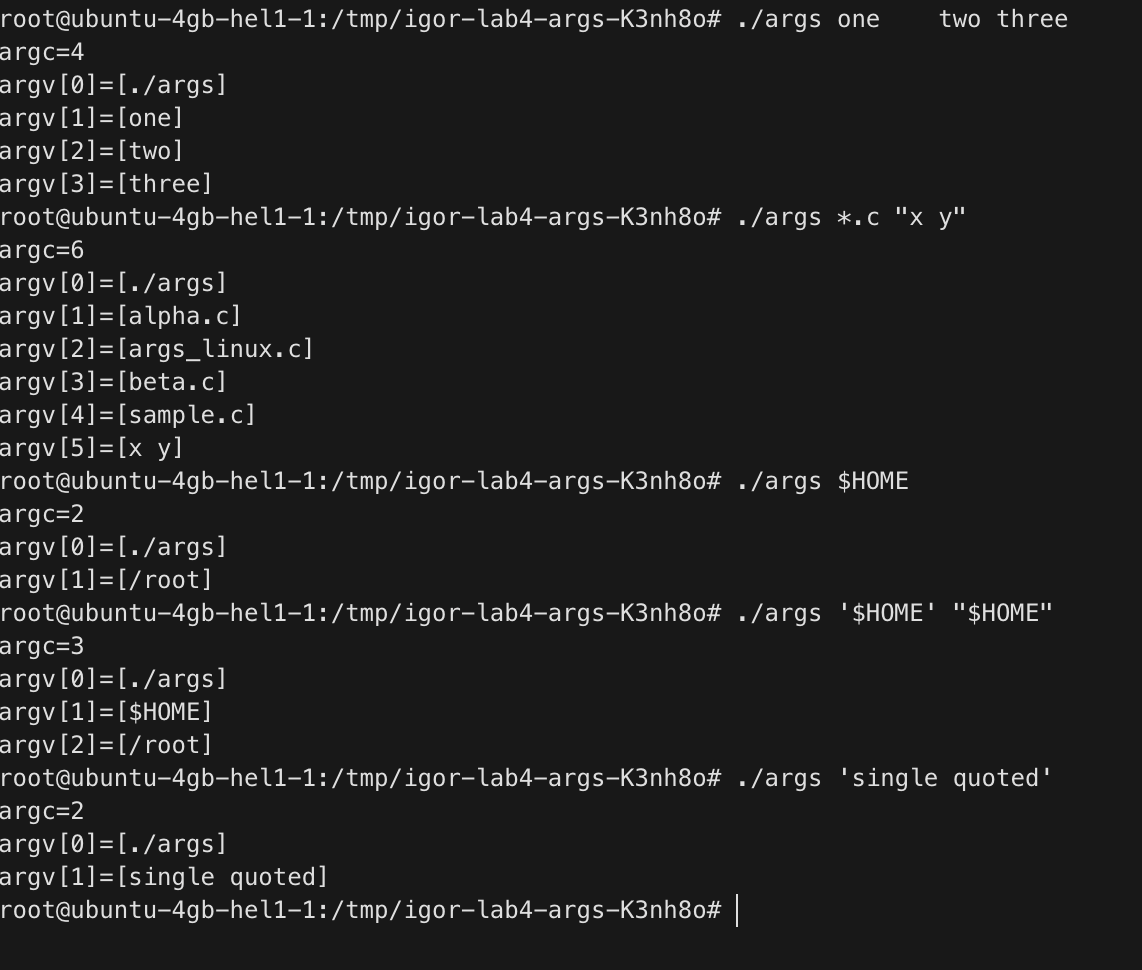
\includegraphics[width=\linewidth,height=0.67\textheight,keepaspectratio]{Lab3-4/evidence/screenshots/lab4-3.3.png}
\end{minipage}\par\medskip

\subsection{Part 4 Reading the
shell}\label{lab4-part-4-reading-the-shell}

This version of user/sh.c has 499 lines. EXEC represents a plain
command; REDIR is introduced by \textless{} or \textgreater; PIPE by
\textbar; LIST by a semicolon; and BACK by ampersand. Parentheses group
a parsed command tree. Cd is recognized in the parent loop before
forking and parsing a general command, so its directory change persists.
The parser has no Bash parameter-expansion or globbing stage, explaining
the literal * and \$HOME results. The five command kinds are visible
both in their definitions and in runcmd dispatch.

\par\medskip\noindent\begin{minipage}{\linewidth}\setstretch{1.0}
\captionof*{figure}{Figura 4.1 – Defined command kinds}
\centering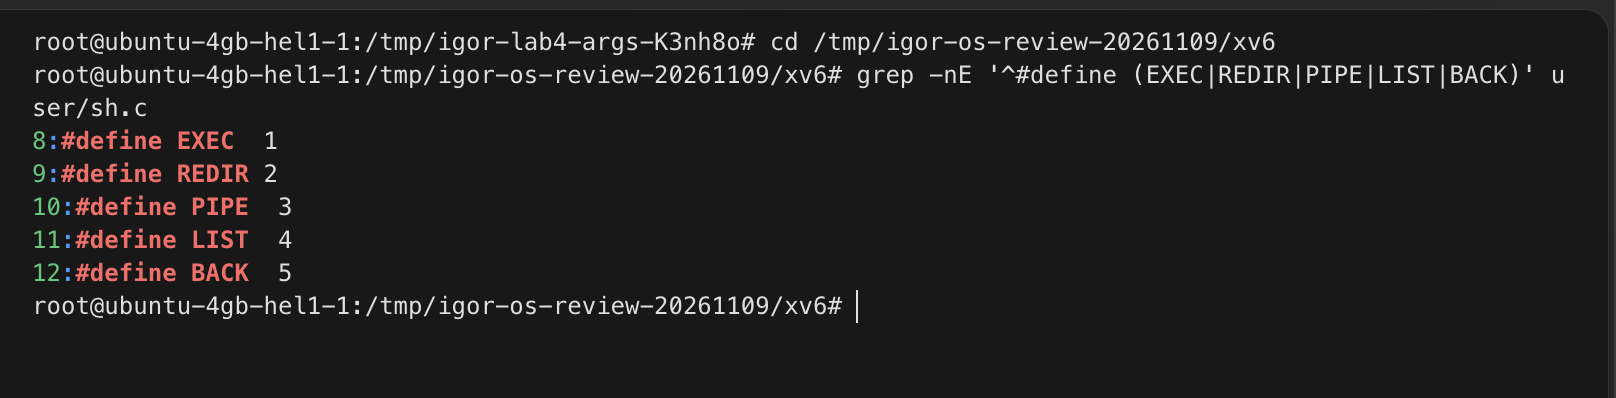
\includegraphics[width=\linewidth,height=0.67\textheight,keepaspectratio]{Lab3-4/evidence/screenshots/lab4-4.1.png}
\end{minipage}\par\medskip

\par\medskip\noindent\begin{minipage}{\linewidth}\setstretch{1.0}
\captionof*{figure}{Figura 4.2 – Dispatch cases}
\centering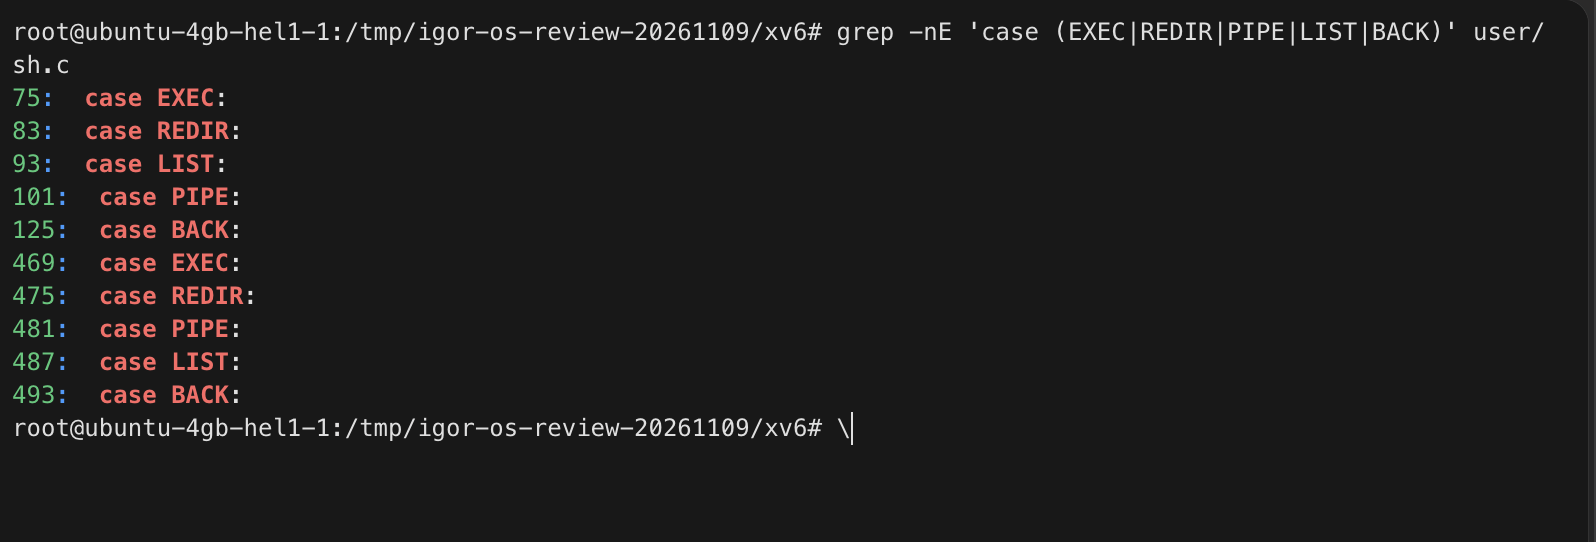
\includegraphics[width=\linewidth,height=0.67\textheight,keepaspectratio]{Lab3-4/evidence/screenshots/lab4-4.2.png}
\end{minipage}\par\medskip

\par\medskip\noindent\begin{minipage}{\linewidth}\setstretch{1.0}
\captionof*{figure}{Figura 4.3 – Parent shell implementation of cd}
\centering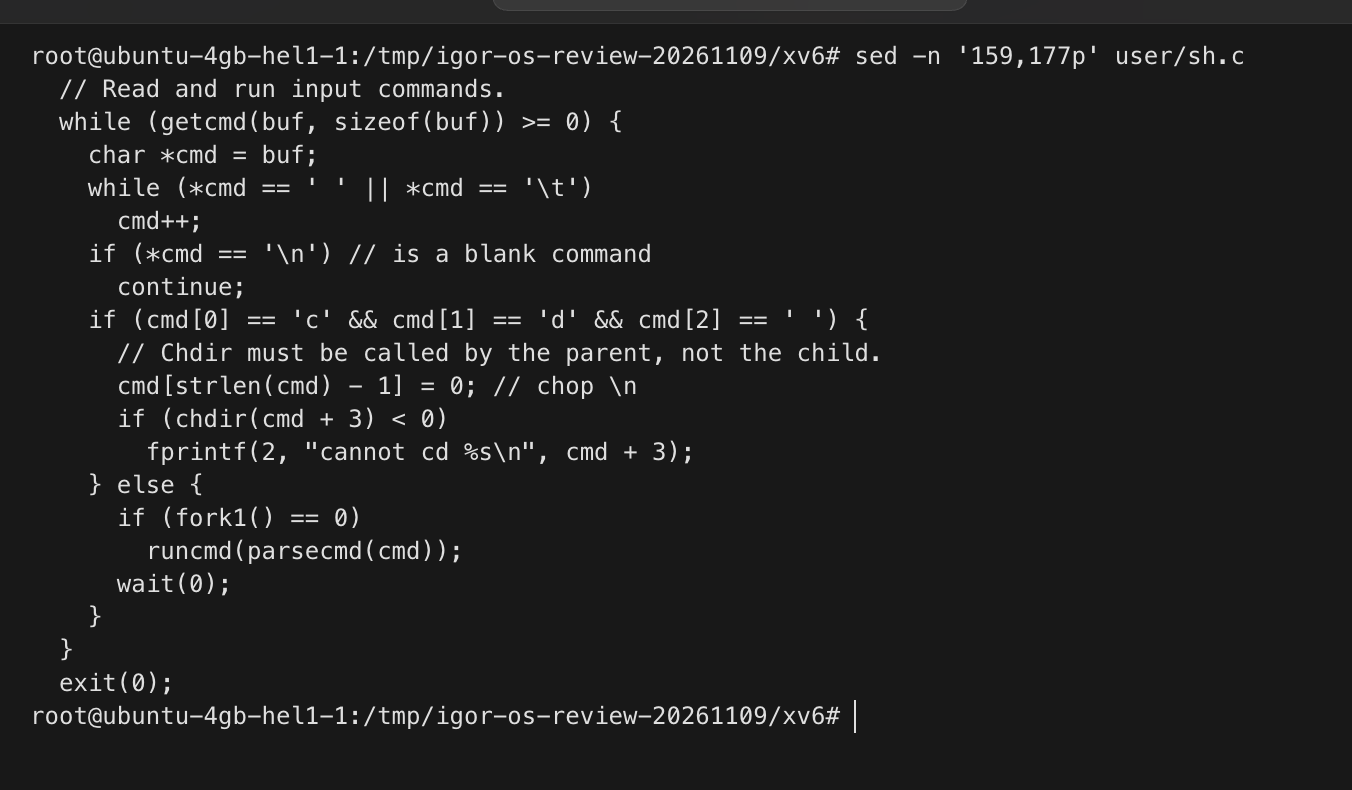
\includegraphics[width=\linewidth,height=0.67\textheight,keepaspectratio]{Lab3-4/evidence/screenshots/lab4-4.3.png}
\end{minipage}\par\medskip

\subsection{Concluziile laboratorului 4}\label{lab4-concluzie}

The two shells share process and descriptor mechanisms but differ before
exec in parsing and expansion. The argument inspector isolates those
differences. The additional cd-list test also shows why a small shell
feature cannot be assumed to compose exactly as in Bash. Both requested
programs and the integrated Makefile are submitted with the full xv6
source and raw console evidence.

\par\noindent\begin{minipage}{\linewidth}

\section{Concluzie}\label{concluzie}

Capturile și scripturile evidențiază distincția dintre transformările
efectuate de shell și argumentele primite de program. Rezultatele
agregării sunt verificabile pe datele de intrare, iar comparația cu xv6
explică de ce aceeași linie poate produce rezultate diferite în două
shell-uri.

\end{minipage}\par

\end{document}
